% Marius-Juston 2026
\documentclass[border=15pt]{standalone}
\usepackage{tikz}
\usetikzlibrary{shapes.geometric, arrows.meta, positioning, calc}

\begin{document}

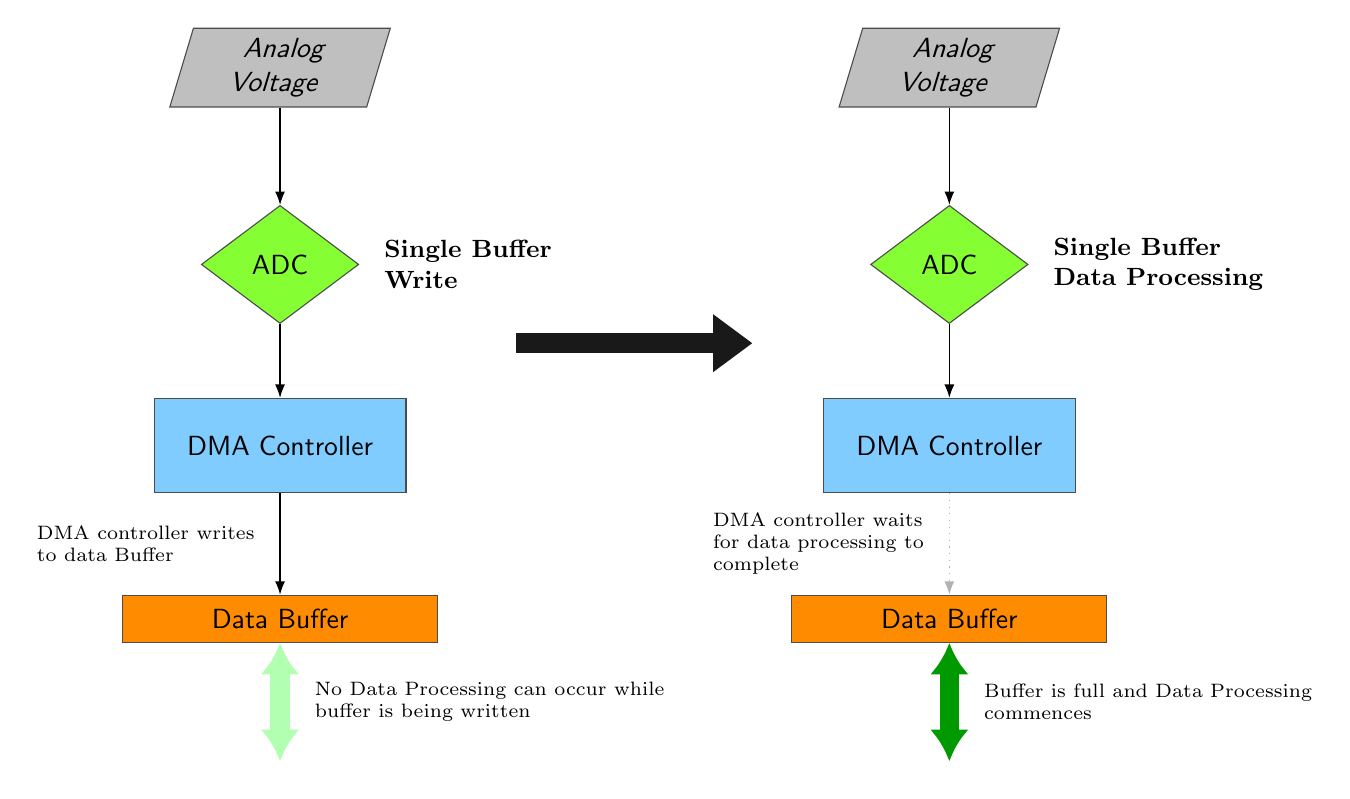
\begin{tikzpicture}[
    font=\sffamily,
    % 1. Core Shapes
    ana/.style={draw=black!70, fill=gray!50, minimum width=2.5cm, minimum height=1cm, xslant=0.3, align=center},
    adc/.style={diamond, aspect=1.3, draw=black!70, fill=green!60!yellow!80, minimum width=2cm, minimum height=1.5cm, align=center},
    dma/.style={draw=black!70, fill=blue!40!cyan!50, minimum width=3.2cm, minimum height=1.2cm, align=center},
    buf/.style={draw=black!70, fill=orange!90!yellow, minimum width=4cm, minimum height=0.6cm, align=center},
    % 2. Routing and Process Arrows
    % Removed 'thick' to make standard communication lines thinner and cleaner
    arr/.style={-Latex},
    waitarr/.style={dotted, draw=gray!60, -Latex},
    bigarr/.style={line width=2.5mm, -{Triangle[length=5mm,width=7mm]}, draw=black!90},
    % Fixed dynamic scaling bug by passing absolute lengths to the arrowheads
    dataproc/.style={line width=2.5mm, draw=green!60!black, {Latex[length=4mm,width=5mm]}-{Latex[length=4mm,width=5mm]}},
    fadedproc/.style={line width=2.5mm, draw=green!30, {Latex[length=4mm,width=5mm]}-{Latex[length=4mm,width=5mm]}}
]

% ===============================
% Stage 1: Single Buffer Write
% ===============================
\begin{scope}[shift={(0,0)}]
    % Explicitly aligning x-coordinates to '0' ensures absolute verticality
    \node[ana] (ana1) at (0, 0) {Analog\\Voltage};
    \node[adc] (adc1) at (0, -2.5) {ADC};
    \node[dma] (dma1) at (0, -4.8) {DMA Controller};
    \node[buf] (buf1) at (0, -7.0) {Data Buffer};

    % Linear Data Flow
    % Routing explicitly from the un-slanted vertical center of the ana1 shape
    \draw[arr] (ana1.center |- ana1.south) -- (adc1.north);
    \draw[arr] (adc1.south) -- (dma1.north);
    
    % DMA to Buffer Write Pipeline
    \draw[arr] (dma1.south) -- (buf1.north) node[midway, left=0.2cm, font=\scriptsize, align=left] {DMA controller writes\\to data Buffer};

    % Data Processing Indicator (Inactive/Locked state)
    \draw[fadedproc] (buf1.south) -- ++(0,-1.5) node[midway, right=0.2cm, font=\scriptsize, text=black, align=left] {No Data Processing can occur while\\buffer is being written};
    
    % Title Assignment
    \node[font=\bfseries\small, align=left, anchor=west] at (1.2, -2.5) {Single Buffer\\Write};
\end{scope}

% State Transition Arrow
\draw[bigarr] (3,-3.5) -- (6,-3.5);

% ===============================
% Stage 2: Single Buffer Data Processing
% ===============================
\begin{scope}[shift={(8.5,0)}]
    % Explicitly aligning x-coordinates to '0' ensures absolute verticality
    \node[ana] (ana2) at (0, 0) {Analog\\Voltage};
    \node[adc] (adc2) at (0, -2.5) {ADC};
    \node[dma] (dma2) at (0, -4.8) {DMA Controller};
    \node[buf] (buf2) at (0, -7.0) {Data Buffer};

    % Linear Data Flow
    \draw[arr] (ana2.center |- ana2.south) -- (adc2.north);
    \draw[arr] (adc2.south) -- (dma2.north);
    
    % DMA to Buffer Wait State (Bottleneck)
    \draw[waitarr] (dma2.south) -- (buf2.north) node[midway, left=0.2cm, font=\scriptsize, text=black, align=left] {DMA controller waits\\for data processing to\\complete};

    % Data Processing Indicator (Active state)
    \draw[dataproc] (buf2.south) -- ++(0,-1.5) node[midway, right=0.2cm, font=\scriptsize, text=black, align=left] {Buffer is full and Data Processing\\commences};
    
    % Title Assignment
    \node[font=\bfseries\small, align=left, anchor=west] at (1.2, -2.5) {Single Buffer\\Data Processing};
\end{scope}

\end{tikzpicture}
\end{document}